Plot the frame G coordinates $(2, -1)_G$ Now express the frame G coordinates $(2, -1)_G$ in the frame M, and confirm that this is the same point by plotting it using the frame M.

\begin{solution}
\begin{align*}
    R_{MG}T_{MG} &= \begin{bmatrix}
        \cos{\frac{\pi}{3}} & \sin{\frac{\pi}{3}} & 0 \\
        -\sin{\frac{\pi}{3}} & \cos{\frac{\pi}{3}} & 0 \\
        0 & 0 & 1 \\
    \end{bmatrix} \begin{bmatrix}
        1 & 0 & 3 \\
        0 & 1 & -1 \\
        0 & 0 & 1 \\
    \end{bmatrix} \\
    &= \begin{bmatrix}
        0.5 & 0.866 & 0.634 \\
        -0.866 & 0.5 & -3.098 \\
        0 & 0 & 1
    \end{bmatrix} \\
    r_M &= R_{MG} T_{MG} r_G \\
    &= \begin{bmatrix}
        0.7679 \\
       -5.3301 \\
        1
    \end{bmatrix} \\
    r_M &= 0.7679 \boldsymbol{\hat{i}}_M - 5.3301 \boldsymbol{\hat{j}}_M
\end{align*}

\begin{center}
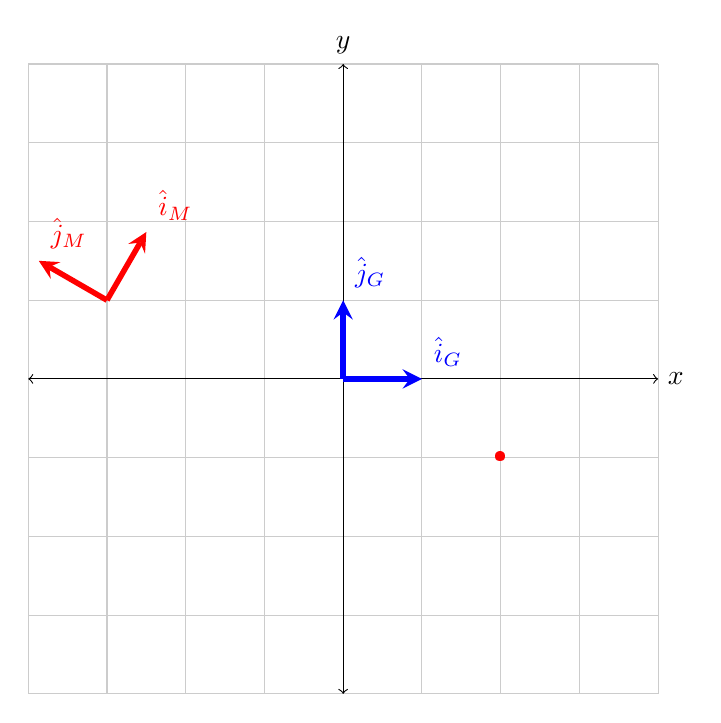
\begin{tikzpicture}    
    \draw[thin,gray!40] (-4,-4) grid (4,4);
    \draw[<->] (-4,0)--(4,0) node[right]{$x$};
    \draw[<->] (0,-4)--(0,4) node[above]{$y$};
    \draw[line width=2pt,blue,-stealth](0,0)--(1,0) node[anchor=south west]{$\boldsymbol{\hat{i}}_G$};
    \draw[line width=2pt,blue,-stealth](0,0)--(0,1) node[anchor=south west]{$\boldsymbol{\hat{j}}_G$};
    \draw[line width=2pt,red,-stealth](-3,1)--(-2.5,1.866) node[anchor=south west]{$\boldsymbol{\hat{i}}_M$};
    \draw[line width=2pt,red,-stealth](-3,1)--(-3.866,1.5) node[anchor=south west]{$\boldsymbol{\hat{j}}_M$};
    \node [red] at (2, -1) {\textbullet};
\end{tikzpicture}
\end{center}
\end{solution}